\documentclass{article}

\textwidth=6.5in
\textheight=8.5in
\voffset=-54pt
\oddsidemargin=0in
\evensidemargin=0in
\setlength{\parskip}{8pt}
\setlength{\parindent}{0pt}

\usepackage{amsmath, amssymb}
\usepackage{ifthen}

\usepackage[inline]{enumitem}
\setlist{topsep=0pt, parsep=8pt}

\usepackage[rgb,table]{xcolor}\convertcolorsUfalse
\usepackage{graphicx}

% change hyperref options
\PassOptionsToPackage{hyphens}{url}
\usepackage[bookmarks,colorlinks,linkcolor=black,citecolor=blue,pdfstartview=FitH,urlcolor=blue]{hyperref}
\hypersetup{pdfpagemode=UseNone}
\usepackage{bookmark}

\usepackage{graphicx}
\usepackage{multicol}
\usepackage{framed}
\usepackage{array}

\usepackage{icomma}

\usepackage{pifont}

\newlist{altenumerate}{enumerate}{3}

\usepackage{soul}

\usepackage{pgfplots}
\pgfplotsset{compat=1.18}  
\pgfplotscreateplotcyclelist{mycolor}{black, blue, red, green!70!black, magenta, purple, cyan, orange }  
\pgfplotsset{
  disabledatascaling,
  cycle list=tikzcolor, 
  axis lines=middle,
  every axis plot/.style={no marks, thick},
  every axis/.style={
    enlarge x limits=false,
    enlarge y limits=auto,
    xlabel style={at={(current axis.right of origin)},anchor=west},
    ylabel style={at={(current axis.above origin)},anchor=south},
    % extra x and y ticks for asymptotes
    extra x tick style={grid=major, grid style={dashed,black}},
    extra y tick style={grid=major, grid style={dashed,black}},
    /pgf/number format/1000 sep={},
  },    
  tick label style = {font=\footnotesize, fill=\currentbgcolor, inner sep=0pt},    
  xticklabel shift=1pt,    
  scaled ticks=false,
  scaled y ticks=false,
  unbounded coords=jump,
  samples=101,
  minor tick length=0,
  scatter/classes={
    open={mark=*,draw=black,fill=white, mark size=2, thin},
    closed={mark=*,draw=black,fill=black, mark size=2, thin}
  },
  width=3in,
}
\pgfplotsset{open/.style={only marks, mark=*, fill=white, thin, mark size=2}}
\pgfplotsset{closed/.style={only marks, mark=*, draw=black, fill=black,
    thin, mark size=2}}
\pgfplotsset{labeled/.style={nodes near coords, only marks, mark=*, draw=black, fill=black, thin, mark size=2, point meta=explicit symbolic}}

\usepackage{tikz}
\usetikzlibrary{
  matrix,%
  % enables the snake paths
  decorations.pathmorphing,%
  % enables bigger arrows
  decorations.markings,%
  decorations.pathreplacing,%
  decorations.text,%
  calc,%
  patterns,%
  shapes.geometric,%
  arrows,
  decorations.shapes,
  positioning,
  plotmarks,
  intersections
}
\tikzset{>=latex} % sets default arrow type in tikz
\tikzset{font=\normalsize}
\tikzset{mark size=1.5pt, mark options=thin}
\tikzset{pin distance=4pt,
  every pin edge/.style={<-, thin, shorten <= -2pt}}

\interfootnotelinepenalty=10000
\renewcommand{\thefootnote}{(\arabic{footnote})}

\usepackage{multirow, bigdelim}

% change to \usepackage[sols]{handout} to see solutions
\usepackage[]{handout}

\newcommand\iscurrentenumi[1]{%
  \ifthenelse{\equal{#1}{\theenumi}}{}{#1}}
\setenumerate[1]{ref=\#\arabic*}
\setenumerate[2]{ref=\protect\iscurrentenumi{\theenumi}(\alph*)}
\newcommand\enumiiprefix[2]{%
  \ifthenelse{{\equal{#1}{\theenumi}}\AND{\equal{#2}{(\alph{enumii})}}}{}{}%
  \ifthenelse{{\equal{#1}{\theenumi}}\AND{\NOT{\equal{#2}{(\alph{enumii})}}}}{#2}{}%
  \ifthenelse{\equal{#1}{\theenumi}}{}{#1#2}%
}
\setenumerate[3]{ref=\protect\enumiiprefix{\theenumi}{(\alph{enumii})}\roman*}

\makeatletter

% underline links               
\let\@href=\href
\renewcommand{\href}[2]{\@href{#1}{\ul{#2}}}

\newdimen\SOUL@dimen %new
\def\SOUL@ulunderline#1{{%
    \setbox\z@\hbox{#1}%
    % \dimen@=\wd\z@
    \SOUL@dimen=\wd\z@ %new
    \dimen@i=\SOUL@uloverlap
    \advance\SOUL@dimen2\dimen@i %\dimen@ exchanged too
    \rlap{%
      \null
      \kern-\dimen@i
      % \SOUL@ulcolor{\SOUL@ulleaders\hskip\dimen@}%
      \SOUL@ulcolor{\SOUL@ulleaders\hskip\SOUL@dimen}% new
    }%
    \unhcopy\z@
  }}

\makeatother

\newcommand{\related}[1]{%
\fcolorbox{black}{yellow}{%
  %\parbox[t]{12pt}{$\clubsuit$}%
  \parbox[t]{\linewidth-8pt}{\emph{Related problems:} #1}}}

\renewcommand{\answer}[1]{#1}

\definecolor{purple}{rgb}{0.5,0,1.0}
\definecolor{hotpink}{rgb}{1, 0, 0.5}

\definecolor{skyblue}{rgb}{0, 0.5, 1}

\newcommand{\highlight}[1]{\boldmath\hl{\textbf{#1}}\unboldmath}

\newcounter{imagecounter}
\newcounter{columncounter}
\newenvironment{imagetable}[3][]{%
  \setcounter{imagecounter}{0}
  \setcounter{columncounter}{#2}
  \addtocounter{columncounter}{-1}
  \newcolumntype{i}{>{\raisebox{-1ex-\height}{\makebox[1em]{\hfill\stepcounter{imagecounter}(#3{imagecounter})}}\hspace{4pt}\begin{minipage}[t]{\linewidth/#2-1em-\tabcolsep*3}\arraybackslash\vspace{0pt}}l<{\end{minipage}}}
\begin{tabular}{i*{\value{columncounter}}{#1i}}}
{\end{tabular}}  

\newcommand{\goal}[1]{\textbf{\textcolor{skyblue}{#1}}}

\usepackage{amsthm}

% make URLs print in the same font
\usepackage{url}
\urlstyle{same}

\usepackage{pifont}
\def\exend{\hfill\ding{118}}

%\makeatletter\@addtoreset{equation}{section}\makeatother
%\renewcommand{\theequation}{\arabic{section}.\arabic{equation}}

\newtheoremstyle{theorem}% name
{8pt}%      Space above
{0pt}%      Space below
{\itshape}%         Body font
{}%         Indent amount (empty = no indent, \parindent = para indent)
{\bfseries}% Thm head font
{.}%        Punctuation after thm head
{.5em}%     Space after thm head: " " = normal interword space;
                                %       \newline = linebreak
{}%         Thm head spec (can be left empty, meaning `normal')

\theoremstyle{theorem}

\let\Theorem\undefined
\newtheorem{Theorem}[equation]{Theorem}
\let\Definition\undefined
\newtheorem{Definition}[equation]{Definition}
\let\Summary\undefined
\newtheorem{Summary}[equation]{Summary}
\let\Conjecture\undefined
\newtheorem{Conjecture}[equation]{Conjecture}
\let\Fact\undefined
\newtheorem{Fact}[equation]{Fact}

\renewcommand{\thesubsection}{\arabic{subsection}}
\makeatletter
\def\@seccntformat#1{\@ifundefined{#1@cntformat}%
   {\csname the#1\endcsname\quad}%       default
   {\csname #1@cntformat\endcsname}}%    enable individual control
\newcommand\section@cntformat{}
\makeatother

  \usepackage{exam}

\usepackage{fancyhdr}
\lhead{\textcolor{white}{This content is protected and may not be shared, uploaded, or distributed.}}
\rhead{}
\rfoot{\vspace*{\fill}\footnotesize\textcopyright{} \emph{Harvard Math Ma}}
\renewcommand{\headrulewidth}{0pt}
\pagestyle{fancy}
\begin{document}

  \title{Final Exam Practice 4}

\instructions{instructions.tex}{}

\listofproblems

\begin{enumerate}
\item \label{fall2015-1a-m1practice3-6} \points{11}  

  \begin{enumerate}
  \item
    \begin{problem}[\vfill]
      Brook has \$2000 that he wants to save, and he decides to put it in
      a bank account that promises his money will grow by 6\% each year.
      Write a formula for $B(t)$, the number of dollars in Brook's account
      after $t$ years (assuming he makes no additional deposits or
      withdrawals).
    \end{problem}

    \begin{solution}
      The amount of money in Brook's account is multiplied by 1.06 each
      year, so in $t$ years, he will have $\boxed{2000 (1.06^t)}$
      dollars. 
    \end{solution}

  \item
    \begin{problem}[\vfill\newpage]
      Robin has \$1000 that she wants to save, and she decides to put it in a bank account that promises her money will grow by 3\% every 6 months. Write a formula for $R(t)$, the number of dollars in Robin's account after $t$ years (assuming she makes no additional deposits or withdrawals).
    \end{problem}

    \begin{solution}

      Let's make a table. Robin's account starts out with \$1000 and grows by 3\% (that is, gets multiplied by $1.03$) every 6 months. Since $t$ is measured in years and 6 months is 0.5 years, here's what happens:
      \begin{center}
        \begin{tabular}{>{$}c<{$} | >{$}c<{$}}
          t (\text{years})& R(t) \\
          \hline
          0 & 1000 \\
          0.5 & 1000 (1.03) \\
          1 & 1000 (1.03^2) \\
          1.5 & 1000  (1.03^3)
        \end{tabular}
      \end{center}
      As we can see, the pattern is $R(t) = \boxed{1000 (1.03^{2t})}$. 
    \end{solution}

  \item
    \begin{problem}[\vfill]
      Is there any time in the future at which Robin and Brook's accounts
      will have the same amount of money?  If so, find such a time; if
      not, explain why not. 
    \end{problem}

    \begin{solution}
      Although Robin starts with less money, her interest rate is actually higher than Brook's. To understand why, think about what happens in just the first year. In the first 6 months, she gets an additional 3\% of \$1000, which is \$30. In the second 6 months, she gets an additional 3\% of \$1030, not 3\% of \$1000. So, she ends up earning a little more than 6\% of \$1000. Therefore, Robin's account will eventually catch up with Brook's. To find when this happens, we solve
      \begin{align*}
        2000 (1.06^t) &= 1000 (1.03^{2t}) \\
        \intertext{Let's divide both sides by 1000 just to make things a
          little simpler:}
        2 (1.06^t) &= 1.03^{2t} \\
        \shortintertext{To get the $t$'s out of the exponents, we'll take
          the natural log of both sides:}
        \ln \left[ 2 (1.06)^t \right] &= \ln \left( 1.03^{2t} \right) \\
        \ln 2 + \ln \left( 1.06^t \right) &= \ln \left( 1.03^{2t} \right)
        \\
        \ln 2 + t \ln 1.06 &= 2t \ln 1.03 \\
        \intertext{This is linear, so we'll put the terms with $t$ on one side and the terms without $t$ on the other:}
        \ln 2 &= 2t \ln 1.03 - t \ln 1.06 \\
        \ln 2 &= t \left( 2 \ln 1.03 - \ln 1.06 \right) \\
        \frac{\ln 2}{2 \ln 1.03 - \ln 1.06} &= t
      \end{align*}
      So, Robin and Brook's accounts will have the same amount of money
      \fbox{in $\displaystyle \frac{\ln 2}{2 \ln 1.03 - \ln 1.06}$ years}
      (this is about 816.72 years).
    \end{solution}

  \item
    \begin{problem}[\nstretch{0.5}]
      Suppose you have some money that you'd like to put in a savings
      account.  Are you better off with Brook's bank or Robin's bank?
      Explain briefly.
    \end{problem}

    \begin{solution}
      As we already said, Robin's account has a higher yearly interest rate than Brook's, so you're better off with \fbox{Robin's bank}.
    \end{solution}

  \end{enumerate}

\item \label{fall2013-ma-premidterm-3} \points{12} 

  In the second half of the twentieth century, the sparrow population in the UK suffered a significant decline. From 1970 to 2000, the sparrow population was decreasing at a slowing rate.

  Surveys estimate that there were 20 million sparrows in 1970 and 10 million sparrows in 2000.

  In 1970, the sparrow population was decreasing at a rate of 500,000 sparrows per year.

  \begin{enumerate} 
  \item
    \begin{problem}[\vfill]
      Sketch a possible graph of the UK sparrow population as a function
      of time, from 1970 to 2000.  Make sure the key characteristics of
      your graph are consistent with the information you have above, and
      label your axes clearly. 
    \end{problem}

    \begin{solution}
      The graph should be decreasing and concave up (because the sparrow population was decreasing at a slowing rate). In addition, the graph should go through points corresponding to 20 million sparrows in 1970 and 10 million sparrows in 2000. In the graph below, we've chosen to make the horizontal axis ``years since 1970'' and the vertical axis ``millions of birds'', but different choices are fine as long as you label them clearly.

      \answer{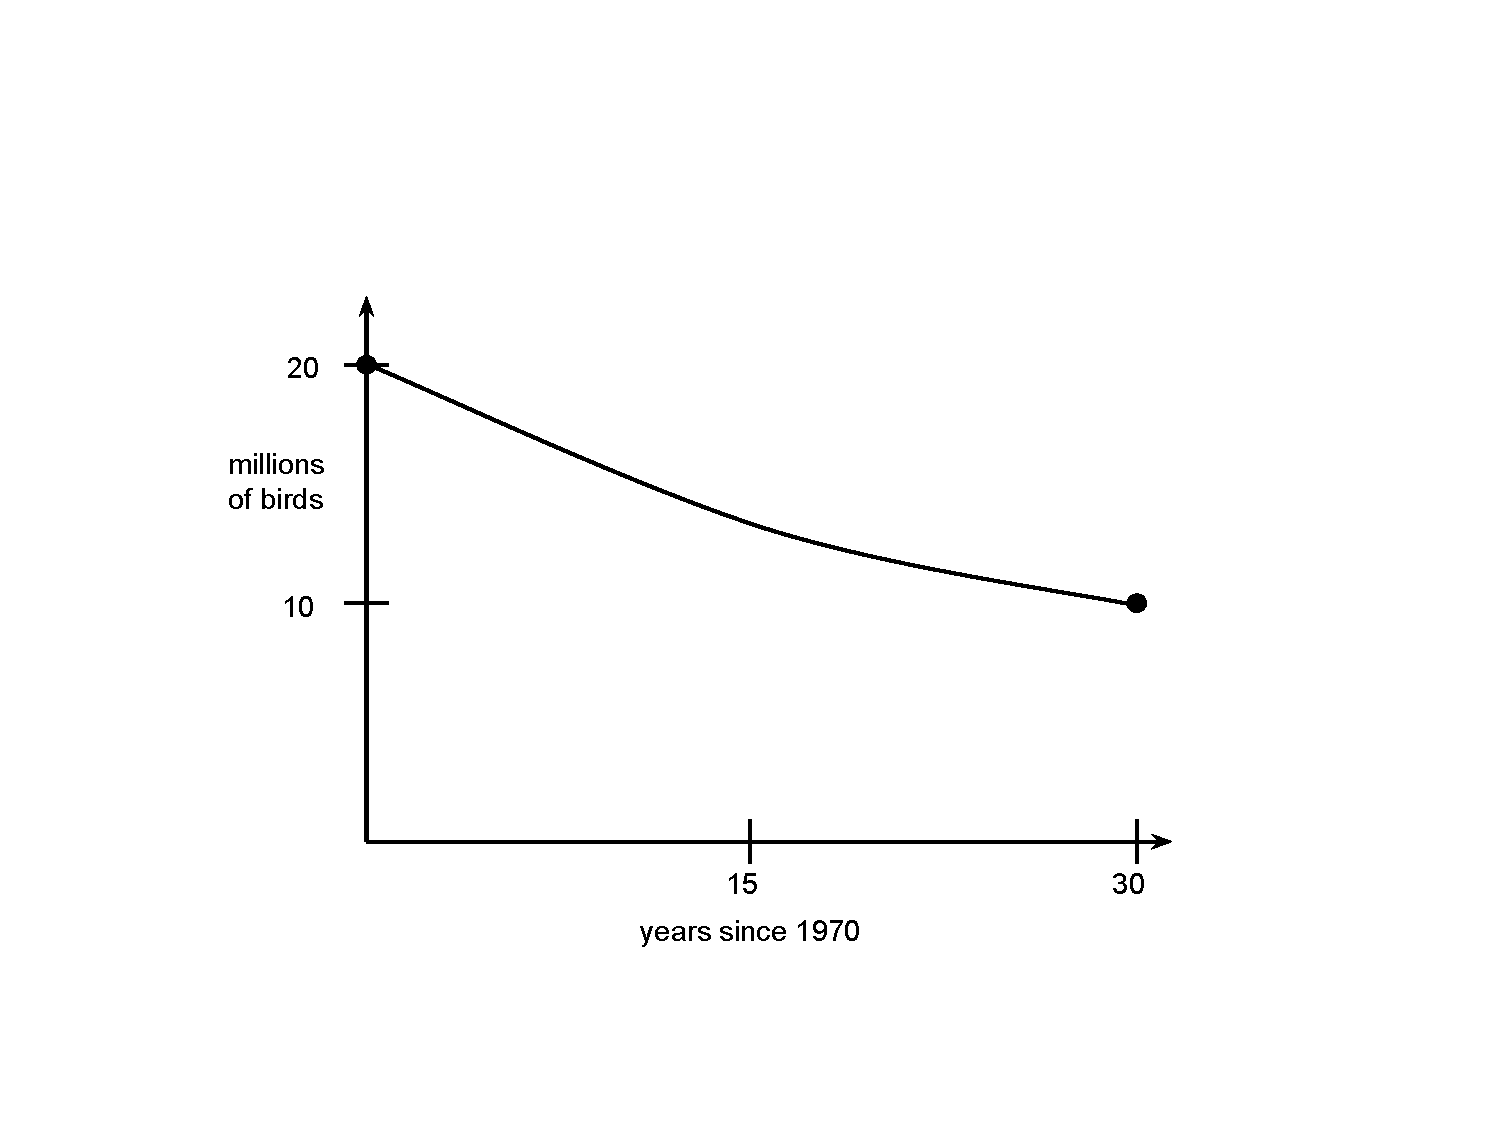
\includegraphics[width=4in]{images/fall2013-ma-premidterm-3a}}
    \end{solution}    

  \item \label{fall2013-ma-premidterm-3b}
    \begin{problem}[\vfill\newpage]
      Use a secant or tangent line approximation to find an upper bound for the number of sparrows in the UK in 1985. Clearly justify your answer using words and/or your graph.
    \end{problem}

    \begin{solution}
      There's only one secant line that we know: the one between the two points we know. As shown on the graph below, this secant line (shown in red) will overestimate the number of birds in 1985.

      The only tangent line we can find is the one at $t = 0$ because the only instantaneous rate of change we're told is the one at $t = 0$. This tangent line (shown in blue) will underestimate the number of birds in 1985.

      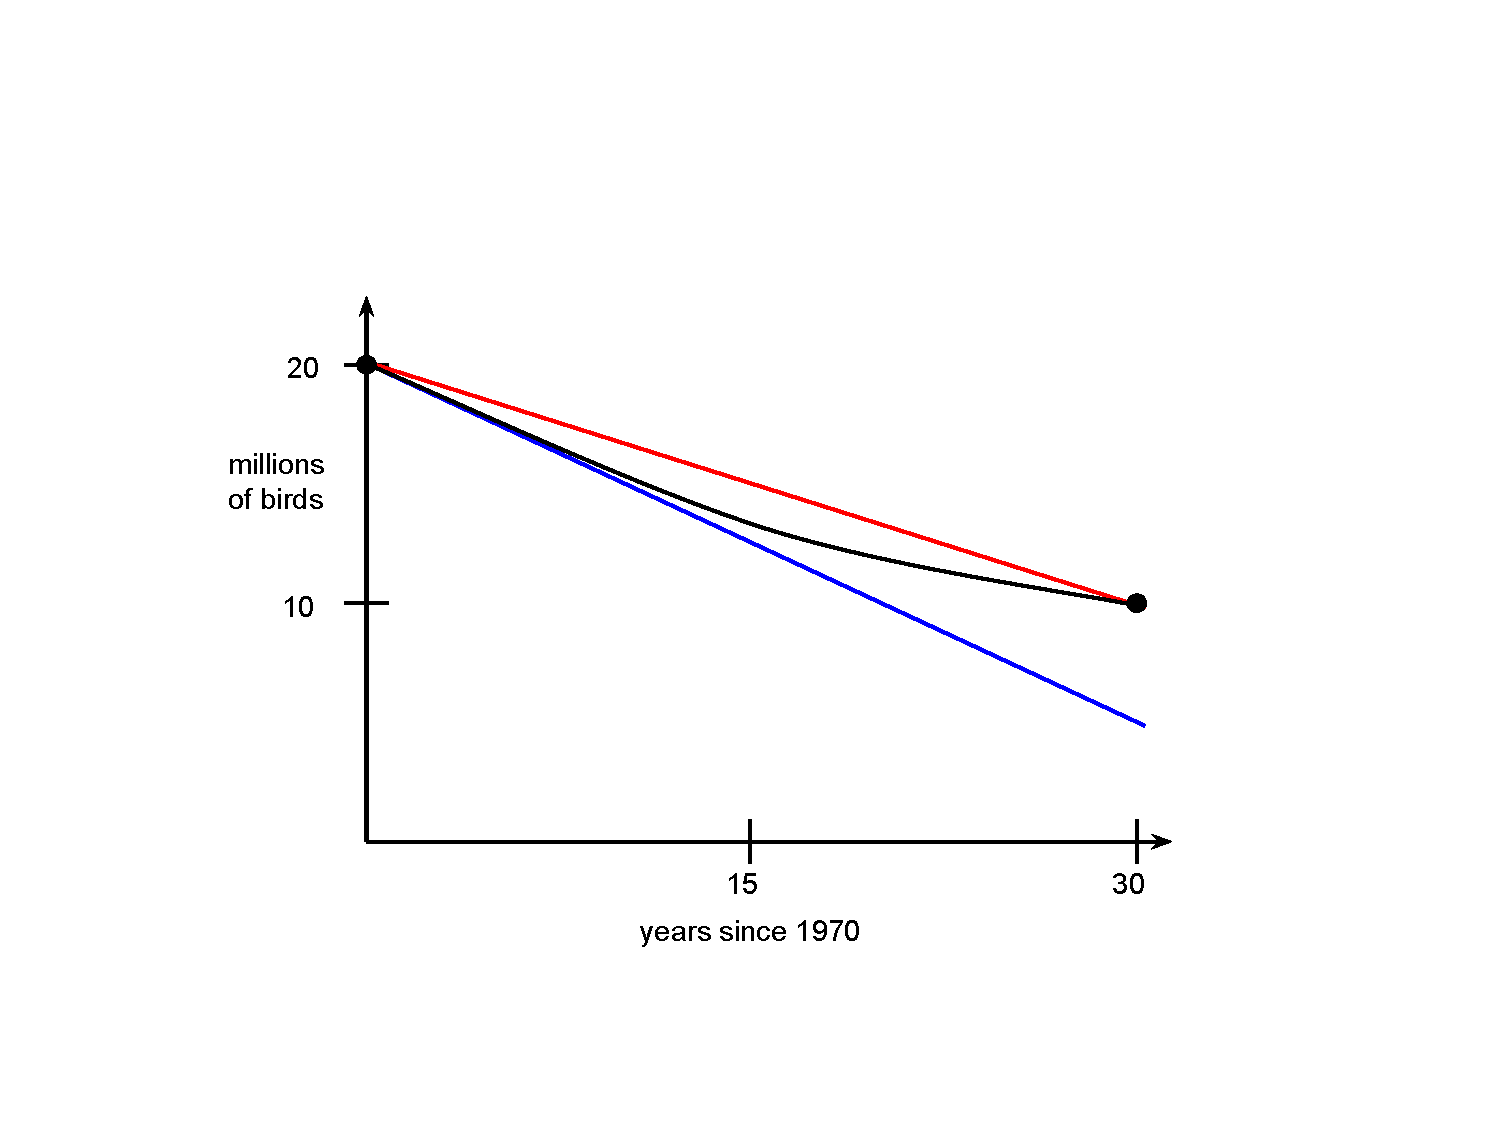
\includegraphics[width=4in]{images/fall2013-ma-premidterm-3b}

      So, to get an upper bound, we should use a secant line approximation. The secant line shown has slope $\frac{10 - 20}{30 - 0} = - \frac{1}{3}$ and includes the point $(0, 20)$, so its equation is $y = -\frac{1}{3} t + 20$. 1985 corresponds to $t = 15$, and the height of the secant line at $t = 15$ is $y = -\frac{1}{3} (15) + 20 = 15$. Therefore, \fbox{15 million birds} is an upper bound for the number of sparrows in the UK in 1985.
    \end{solution}

  \item
    \begin{problem}[\vfill]
      Use a secant or tangent line approximation to find a lower bound for the number of sparrows in the UK in 1985. Clearly justify your answer using words and/or your graph.
    \end{problem}

    \begin{solution}
      Now, we'd like to use the tangent line at $t = 0$, since we saw in \ref{fall2013-ma-premidterm-3b} that it would give an underestimate. The slope of this tangent line is the instantaneous rate of change of the sparrow population in 1970, or $-500,000$ sparrows per year; since we're working in millions of sparrows, we should rewrite this as a slope of $-\frac{1}{2}$ million sparrows per year. The tangent line includes the point $(0, 20)$, so its equation is $y = -\frac{1}{2} t + 20$. Plugging in $t = 15$, we get $y = -\frac{1}{2}(15) +20 = $ \fbox{12.5 million birds} as a lower bound.
    \end{solution}

  \item
    \begin{problem}[\vfill\newpage]
      Is it possible that the sparrow population was declining at 350,000
      sparrows per year in 2000?  Why or why not?
    \end{problem}

    \begin{solution}
      This is \fbox{not possible}.  Here are two different ways to see this:
      \begin{itemize}
      \item \emph{Graphically:} We can see from our graph that the slope
        of the tangent line at $t = 30$ (corresponding to the year 2000)
        must be less steep than the slope of the secant line we drew.  We
        already found that the slope of this secant line was
        $-\frac{1}{3}$ million sparrows per year.

      \item \emph{In context:} If, in 2000, the sparrow population was declining at 350,000 sparrows per year, then it must have been declining at $\geq$ 350,000 sparrows per year for the entire time between 1970 and 2000 (because the sparrow population was decreasing at a slowing rate during this time). But, if it were decreasing at $\geq$ 350,000 sparrows per year for these 30 years, then the population must have fallen by at least (350,000 sparrows/year)(30 years) = 10,500,000 sparrows between 1970 and 2000. However, we are told that the population only fell by 10 million sparrows.
      \end{itemize}
    \end{solution}

  \end{enumerate}

\item \points{17} 

  Let $f(x) = \dfrac{x^2}{e^x}$.

  \begin{enumerate}
  \item
    \begin{problem}[0.25in]
      What's the domain of $f$? 
    \end{problem}

    \begin{solution}
      Both $x^2$ and $e^x$ are defined for all real numbers. And $e^x$ is always positive, so there's no issue with dividing by it. So, the domain is $\boxed{(-\infty, \infty)}$.
    \end{solution}

  \item
    \begin{problem}[\vfill\newpage]
      Does $f$ have a global minimum on its domain? If so, where? If not, why not? How about a global maximum? Justify carefully and completely. 
    \end{problem}

    \begin{solution}
      We'll start by finding critical points. We can rewrite $f(x) = x^2 e^{-x}$. By the Product Rule,
      \[ f'(x) = 2x e^{-x} + x^2 (-e^{-x}) = (2x - x^2) e^{-x} = x (2 - x) e^{-x}.\]
      Since $e^{-x}$ is never 0, the critical points are $x = 0, 2$.

      Since there is more than one critical point, we need to compare the value of $f$ at the critical points with the end behavior. Let's start with the end behavior. Since $x^2 \ll e^x$, $\displaystyle \lim_{x \to \infty} \frac{x^2}{e^x} = 0$. As $x \to -\infty$, $x^2 \to \infty$ while $e^x \to 0$. Since $e^x$ is always positive, $\displaystyle \lim_{x \to \infty} \frac{x^2}{e^x} = \infty$. So, we have:      
      \begin{align*}
        \lim_{x \to \infty} f(x) &= 0 \\
        \lim_{x \to -\infty} f(x) &= \infty \\
        f(0) &= 0 \\
        f(2) &= \dfrac{4}{e^2}
      \end{align*}
      So, $f$ \fbox{doesn't have a global maximum on $(-\infty, \infty)$}, and it has a \fbox{global minimum at $x = 0$}.       
    \end{solution}

  \item
    \begin{problem}[\vfill]
      Where is $f$ concave up? Where is $f$ concave down?
    \end{problem}

    \begin{solution}
      We'll make a sign chart for $f''$. Since $f'(x) = (2x - x^2) e^{-x}$, the Product Rule gives
      \[ f''(x) = (2 - 2x) e^{-x} + (2x - x^2) (-e^{-x}) = (2 - 2x - 2x + x^2) e^{-x} = (x^2 - 4x + 2) e^{-x}.\] This is never undefined. Since $e^{-x}$ is never 0, $f''(x) = 0$ when $x^2 - 4x + 2 = 0$. By the quadratic formula, this is when $x = \dfrac{4 \pm \sqrt{16 - 8}}{2} = \dfrac{4 \pm 2 \sqrt{2}}{2} = 2 \pm \sqrt{2}$. Now, we need to test 3 points:
      \begin{itemize}
      \item First, we need to test a point less than $2 - \sqrt{2}$. Since $\sqrt{2} < 2$, we can be sure $0 < 2 - \sqrt{2}$. We have $f''(0) = 2 > 0$.
      \item Next, we need to test a point between $2 - \sqrt{2}$ and $2 + \sqrt{2}$; the obvious choice is $2$. We have $f''(2) = -2e^{-2} < 0$.
      \item Finally, we need to test a point greater than $2 + \sqrt{2}$. Since $\sqrt{2} < 2$, we can use 4. We have $f''(4) = 2 e^{-4} > 0$. 
      \end{itemize}
      So, here's our sign chart for $f''$:
      \begin{center}
        \begin{tikzpicture}
          \begin{axis}[axis y line=none, x axis line style={-}, xtick={0.585786, 3.41421}, xticklabels={$2-\sqrt{2}$, $2+\sqrt{2}$}, ymin=-2, height=1in, width=3in, clip=false]
            \addplot+[domain=-5.07107:6.24264, very thin]{0};
            \draw (-5.07107, -1.5) node[right] {sign of $f''$};
            \draw (-0.828427, -1.5) node{$+$};%
            \draw (2, -1.5) node{$-$};%
            \draw (4.82843, -1.5) node{$+$};%
          \end{axis}
        \end{tikzpicture}
      \end{center}
      Therefore, $f$ is \fbox{concave up on $(-\infty, 2 - \sqrt{2}) \cup (2 + \sqrt{2}, \infty)$ and concave down on $(2 - \sqrt{2}, 2 + \sqrt{2})$}.
    \end{solution}

  \item
    \begin{problem}[\nstretch{0.5}]
      Sketch a graph of $f$. 
    \end{problem}

    \begin{solution}
      Let's start with what we figured out in (b): we calculated $f(0)$, $f(2)$, $\displaystyle \lim_{x \to \infty} f(x)$ and $\displaystyle \lim_{x \to -\infty} f(x)$. Let's mark these on our graph:
      \begin{center}
        \begin{tikzpicture}
          \begin{axis}[xtick={0, 2}, ytick={4/e^2}, yticklabel={$4/e^2$}, width=2.5in, enlarge y limits=false]
            \addplot+[domain=-3: -2.9] {(x+2)^2/e^(x+2)};
            \addplot+[domain=6:8] {x^2/e^x};
            \addplot+[closed] coordinates { (0, 0) (2, 4/e^2)}; 
          \end{axis}
        \end{tikzpicture}
      \end{center}
      Since $x = 0$ and $x = 2$ are the only critical points, these are the only places where $f$ can switch from increasing to decreasing or vice versa. So, we can see that $f$ must be decreasing on $(-\infty, 0)$, increasing on $(0, 2)$, and decreasing on $(2, \infty)$. I'll draw this in with dotted lines; this is just a first draft that doesn't take concavity into account yet: 
      \begin{center}
        \begin{tikzpicture}
          \begin{axis}[xtick={0, 2}, ytick={4/e^2}, yticklabel={$4/e^2$}, width=2.5in, enlarge y limits=false]
            \addplot+[domain=-3: -2.9] {(x+2)^2/e^(x+2)};
            \addplot+[domain=6:8] {x^2/e^x};
            \addplot+[closed] coordinates { (0, 0) (2, 4/e^2)};
            \addplot+[sharp plot, dotted, black!50!white] coordinates {(-2.9, {0.9^2 / e^(-0.9)}) (0, 0) (2, 4/e^2) (6, 36/e^6)};
          \end{axis}
        \end{tikzpicture}
      \end{center}
      Finally, we'll take concavity into account:      
      \begin{center}
        \answer{
          \begin{tikzpicture}
            \begin{axis}[xtick={0, 2, 2-sqrt(2), 2+sqrt(2)}, xticklabels={$0$, $2\vphantom{\sqrt{2}}$, $2 - \sqrt{2}$, $2 + \sqrt{2}$}, ytick={4/e^2}, yticklabel={$4/e^2$}, width=2.5in, enlarge y limits=false, ]
              \addplot+[domain=-1:8] {x^2/e^x}; 
            \end{axis}
          \end{tikzpicture}
        }
      \end{center}
    \end{solution}

  \end{enumerate}

\item \label{fall2006-1a-midterm1-9-modified} \points{9} 

  At the water cooler, you take a paper cup shaped like a cone from the dispenser and fill it with water at a constant rate of 35 grams per second. (The tip of the cone is the bottom of the cup.) It takes 5 seconds to fill the cone. Let $f(t)$ be the \emph{height} of the water in your paper cone after $t$ seconds of filling.

  \begin{enumerate}
  \item
    \begin{problem}[0.25in]
      What's the domain of $f$? 
    \end{problem}

    \begin{solution}
      Since it takes $5$ seconds to fill the cone, the domain is $\boxed{[0, 5]}$. 
    \end{solution}
  \end{enumerate}

  In the following 3 statements, fill in the blank with ``$<$'', ``$=$'', or ``$>$'', as appropriate. Then justify your answer with sentences.

  \begin{enumerate}[resume]
  \item

    \begin{problem}[\vfill]
      $f(1) \cfitb{0.5in}{<} f(4)$

      \probonly{\textbf{Justification:}}
    \end{problem}

    \begin{solution}
      $f(1)$ represents the water level after 1 second of pouring; $f(4)$
      is the water level after 4 seconds of pouring.  Since you're always
      pouring water into the cup, the water level is higher after 4
      seconds than it is after 1 second.  
    \end{solution}

  \item
    \begin{problem}[\vfill]
      $f'(1) \cfitb{0.5in}{>} f'(4)$

      \probonly{\textbf{Justification:}}
    \end{problem}

    \begin{solution}
      $f'(1)$ represents the rate at which the water level is rising after
      1 second; $f'(4)$ is the rate at which the water level is rising
      after 4 seconds.  Although you're pouring water in at a constant
      rate of 35 grams per second, the bottom of the cone is skinnier than
      the top; therefore, the water level rises more quickly at first and
      gradually slows down.
    \end{solution}

  \item
    \begin{problem}[\vfill\newpage]
      $\frac{f(4)-f(1)}{3} \cfitb{0.5in}{<} f'(1)$

      \probonly{\textbf{Justification:}}
    \end{problem}       

    \begin{solution}
      $\frac{f(4)-f(1)}{3}$ represents the average rate of change in water
      level between 1 second and 4 seconds.  This will be slower than the
      the rate at which the cup was filling at 1 second (i.e. $f'(1)$), 
      since the water level rises more quickly at first and gradually
      slows down.
    \end{solution}

  \end{enumerate}

\item \label{fall2018-final-practice3-6} \points{11} 

  \begin{enumerate}

  \item
    \begin{problem}
      The figure below has two points marked: $(p, \ln p)$ and $(q, \ln q)$. Draw the graph of the function $f(x) = \ln x$, which goes through these two points, and \textbf{label all intercepts}. 
    \end{problem}

    \begin{problemonly}
      \begin{center} 
        \begin{tikzpicture} 
          \begin{axis}[xmin=-6, xmax=6, ymin=-6, ymax=6, clip=false, xtick=\empty, ytick=\empty, enlarge y limits=false, width=6in]
            \addplot+[closed] coordinates { (0.5, {ln(0.5)})} node[anchor=north west] {$(q, \ln q)$}; %
            \addplot+[closed] coordinates { (2.5, {ln(2.5)}) } node[anchor=north west] {$(p, \ln p)$}; %
          \end{axis}
        \end{tikzpicture}
      \end{center} 
    \end{problemonly}

    \begin{solution}
      $f(x) = \ln x$ has no $y$-intercept; its only $x$-intercept is 1. 
      \begin{center} 
        \answer{
          \begin{tikzpicture} 
            \begin{axis}[xmin=-6, xmax=6, ymin=-6, ymax=6, clip=false, xtick={1}, ytick=\empty, enlarge y limits=false]
              \addplot+[domain=1/e^6:6] {ln(x)};
              \addplot+[closed] coordinates { (0.5, {ln(0.5)})} node[anchor=north west] {$(q, \ln q)$}; %
              \addplot+[closed] coordinates { (2.5, {ln(2.5)}) } node[anchor=north west] {$(p, \ln p)$}; %
            \end{axis}
          \end{tikzpicture}
        }
      \end{center} 
    \end{solution}

  \item

    In each part, you're given an expression. Sketch a line on your graph in (a) whose slope is the given expression, and label the line with the letter of the part (A, B, or C). 

    \solonly{\related{{{\#4}} on \href{https://people.math.harvard.edu/~jjchen/mathma/docs/worksheets/worksheet09-sols.html}{the worksheet ``Definition and Interpretation of the Derivative''}; \href{https://people.math.harvard.edu/~jjchen/mathma/docs/homework/PS09.html}{Problem Set 9}, {{\#3}}; {{\#3}} on \href{https://people.math.harvard.edu/~jjchen/mathma/docs/worksheets/worksheet15-sols.html}{the worksheet ``Exam 1 Practice''}}}

    \begin{altenumerate}[label=\Alph*.]
    \item
      \begin{problem}
        $\displaystyle \frac{\ln p - \ln q}{p-q}$
      \end{problem}

      \begin{solution}
        This is the slope of the secant line between $x = p$ and $x = q$. See the sketch in C. 
      \end{solution}

    \item
      \begin{problem}
        $\displaystyle \lim_{s\to q}\frac{\ln q - \ln s}{q-s}$
      \end{problem}

      \begin{solution}
        $\dfrac{\ln q - \ln s}{q - s}$ is the slope of the secant line between $x = q$ and $x = s$. As $s \to q$, this approaches the slope of the tangent line at $x = s$. 
      \end{solution}

    \item
      \begin{problem}
        $\displaystyle \lim_{s\to p} \frac{\ln (p+s) - \ln p}{s}$
      \end{problem}

      \begin{solution}
        $\dfrac{\ln (p+s) - \ln p}{s}$ is the slope of the secant line between $x = p$ and $x = p + s$. As $s \to p$, $p + s \to 2p$, so this is just the slope of the secant line between $x = p$ and $x = 2p$. 

        Here are the 3 slopes: 
        \begin{center}
          \begin{tikzpicture}
            \begin{axis}[xmin=-6, xmax=6, ymin=-6, ymax=6, clip=false, xtick={2.5, 5}, xticklabels={$p$,$2p$}, ytick=\empty, enlarge y limits=false, width=5in]
              \addplot+[domain=1/e^6:6] {ln(x)}; %
              \addplot+[closed] coordinates { (0.5, {ln(0.5)})} node[anchor=north west] {$(q, \ln q)$}; %
              \addplot+[closed] coordinates { (2.5, {ln(2.5)}) } node[anchor=north west] {$(p, \ln p)$}; %
              \addplot+[closed] coordinates { (5, {ln(5)}) }; % 
              \addplot+[sharp plot, hotpink] coordinates { (0.5, {ln(0.5)}) (2.5, {ln(2.5)})} node[pos=0.5, anchor=north west, yshift=-1pt, xshift=1.5pt, fill=white, inner sep=0pt]{A}; %
              \addplot+[domain=0:1.5, skyblue] {2*(x-0.5)+ln(0.5)} node[above]{B}; %
              \addplot+[sharp plot, green!80!black] coordinates { (5, {ln(5)}) (2.5, {ln(2.5)})} node[pos=0.5, anchor=north west, yshift=-1pt, xshift=0.5pt, fill=white, inner sep=0pt]{C}; %
            \end{axis}
          \end{tikzpicture}
        \end{center}
      \end{solution}

    \end{altenumerate}

    \answeronly{
      \begin{tikzpicture}
        \begin{axis}[xmin=-6, xmax=6, ymin=-6, ymax=6, clip=false, xtick={2.5, 5}, xticklabels={$p$,$2p$}, ytick=\empty, enlarge y limits=false, width=5in]
          \addplot+[domain=1/e^6:6] {ln(x)}; %
          \addplot+[closed] coordinates { (0.5, {ln(0.5)})} node[anchor=north west] {$(q, \ln q)$}; %
          \addplot+[closed] coordinates { (2.5, {ln(2.5)}) } node[anchor=north west] {$(p, \ln p)$}; %
          \addplot+[closed] coordinates { (5, {ln(5)}) }; % 
          \addplot+[sharp plot, hotpink] coordinates { (0.5, {ln(0.5)}) (2.5, {ln(2.5)})} node[pos=0.5, anchor=north west, yshift=-1pt, xshift=1.5pt, fill=white, inner sep=0pt]{A}; %
          \addplot+[domain=0:1.5, skyblue] {2*(x-0.5)+ln(0.5)} node[above]{B}; %
          \addplot+[sharp plot, green!80!black] coordinates { (5, {ln(5)}) (2.5, {ln(2.5)})} node[pos=0.5, anchor=north west, yshift=-1pt, xshift=0.5pt, fill=white, inner sep=0pt]{C}; %
        \end{axis}
      \end{tikzpicture}
    }

    \pspace{\newpage}

  \item % added 2023

    \begin{problem}[\vfill]
      Solve $\dfrac{\ln(p + 2) - \ln p}{2} = 3$ for $p$.
    \end{problem}

    \begin{solution}
      \begin{align*}
        \dfrac{\ln(p + 2) - \ln p}{2} &= 3 \\
        \ln (p + 2) - \ln p &= 6 \\
        \ln \left( \frac{p + 2}{p} \right) &= 6 \\
        \intertext{Raising $e$ to both sides,}
        \frac{p + 2}{p} &= e^6 \\
        p + 2 &= e^6 p \\
        \intertext{This equation is linear, so we'll move all the terms with $p$ to one side and all the terms without $p$ to the other:}
        2 &= e^6 p - p \\
        2 &= (e^6 - 1) p \\
        \frac{2}{e^6 - 1} &= p
      \end{align*}
      Since the original equation involved logs, we should check that our solution is in the domain. Our value of $p$ is positive, so both $\ln p$ and $\ln(p + 2)$ are defined. So, $\boxed{\frac{2}{e^6 - 1}}$ is really a solution. 
    \end{solution}

  \end{enumerate}

\item \points{10} 

  \begin{enumerate}
  \item
    \begin{problem}[\nstretch{0.5}]
      If $p(x)$ is a polynomial with 4 turning points, which of the following are possible degrees of $p(x)$? Circle all, and explain your reasoning. 

      \begin{multicols}{4}
        \begin{enumerate}[label=\maybecircle{\Alph*.}]
        \plainitem 4
        \circleitem 5
        \plainitem 6
        \circleitem 7
        \end{enumerate}        
      \end{multicols}
    \end{problem}

    \begin{solution}      
      If $p(x)$ has 4 turning points, then $p'(x)$ must have at least 4 roots, so $p'$ has degree $\geq 4$. Therefore, $p$ has degree $\geq 5$. \answeronly{5,7}

      Since $p(x)$ is a polynomial with 4 turning points, $\displaystyle \lim_{x \to -\infty} p(x) = - \lim_{x \to \infty} p(x)$. (See the example below.) After all, if $p(x)$ ``starts out'' increasing (when $x$ is very negative), after it's turned around 4 times, it will be increasing again; similarly, if $p(x)$ ``starts out'' decreasing, after it's turned around 4 times, it will be decreasing again.

      The fact that $\displaystyle \lim_{x \to -\infty} p(x) = - \lim_{x \to \infty} p(x)$ means $p(x)$ must have odd degree. 
      \begin{center}
        \begin{tikzpicture}
          \begin{axis}[xtick=\empty, ytick=\empty, title={example of polynomial with 4 turning points}, width=2.5in]
            \addplot+[domain=-2.6:2.6] {4*x - (5*x^3)/3 + x^5/5}; 
          \end{axis}
        \end{tikzpicture}
      \end{center}
    \end{solution}

  \item
    \begin{problem}[\vfill]
      Give an example of a degree 6 polynomial that's invertible, or explain why this is impossible. 
    \end{problem}

    \begin{solution}
      This is \fbox{impossible}. If $p(x)$ is a degree 6 polynomial, then $\displaystyle \lim_{x \to -\infty} p(x) = \lim_{x \to \infty} p(x) = \pm \infty$. Therefore, it's impossible for $p(x)$ to pass the horizontal line test. Here are two examples of degree 6 polynomials:
      \begin{center}
        \begin{tikzpicture}
          \begin{axis}[xtick=\empty, ytick=\empty, width=2.25in]
            \addplot+[domain=-2:2] {x^6}; 
          \end{axis}
        \end{tikzpicture}
        \hspace{0.25in}
        \begin{tikzpicture}
          \begin{axis}[xtick=\empty, ytick=\empty, width=2.25in]
            \addplot+[domain=-2.2:3.2] {(3 - x)*(-2 + x)*(-1 + x)*x*(1 + x)*(2 + x)}; 
          \end{axis}
        \end{tikzpicture}
      \end{center}
    \end{solution}

  \item
    \begin{problem}[\vfill\newpage]
      Give an example of a degree 4 polynomial $p(x)$ such that both of the following are true, or explain why this is impossible.
      \begin{itemize}[nosep]
      \item $p''(1) = 0$
      \item $1$ is not an inflection point of $p$.
      \end{itemize}
      \emph{Hint:} What can you say about $p''(x)$? 
    \end{problem}

    \begin{solution}
      An inflection point is where concavity changes, so $p''$ changes sign. Thus, we want $p''(1) = 0$, but we don't want $p''$ to change sign at $x = 1$.

      Since $p(x)$ has degree 4, $p'(x)$ has degree 3, and $p''(x)$ has degree 2. So, we could have $p''(x)$ look like this parabola:
      \begin{center}
        \begin{tikzpicture}
          \begin{axis}[xtick={1}, ytick=\empty, width=2in]
            \addplot+[domain=-1:3] {(x-1)^2}; 
          \end{axis}
        \end{tikzpicture}
      \end{center}
      A possible formula for $p''(x)$ is $p''(x) = (x - 1)^2 = x^2 - 2x + 1$. Working backwards, we can think of a possible $p'(x)$ that has $x^2 - 2x + 1$ as its derivative: $p'(x) = \dfrac{x^3}{3} - x^2 + x$. Working backwards again, we can think of a possible $p(x)$: $p(x) = \boxed{\dfrac{x^4}{12} - \dfrac{x^3}{3} + \dfrac{x^2}{2}}$. 
    \end{solution}

  \end{enumerate}

\item \points{9} 

  \begin{enumerate}
  \item % added 2023
    \begin{problem}[\vfill]
      Evaluate $\displaystyle \lim_{x \to 1^+} \frac{\ln \left( \frac{x}{2} \right)}{x^5-x^4}$, and justify your answer. 
    \end{problem}

    \begin{solution}
      As $x \to 1^+$, the numerator approaches $\ln \left( \frac{1}{2} \right)$ and the denominator approaches 0. Since the numerator approaches a non-zero number while the denominator approaches 0, we need to think about the sign of the numerator and denominator.

      When $x$ is just a bit bigger than 1, the denominator $x^5 - x^4 = x^4 (x - 1)$ is just a bit bigger than 0. On the other hand, the numerator is close to $\ln \left( \frac{1}{2} \right)$, which is a negative number.\footnote{One way to see this is to think about the graph of $\ln x$. Another way is to remember that $\ln \left( \frac{1}{2} \right)$ is the power you raise $e$ to in order to get $\frac{1}{2}$. If you raise $e$ to a positive power, you end up with a number $> 1$, so you must raise $e$ to a negative power in order to get $\frac{1}{2}$.} So, $\dfrac{\ln \left( \frac{x}{2} \right)}{x^5-x^4}$ will be very negative.

      Thus, $\displaystyle \lim_{x \to 1^+} \frac{\ln \left( \frac{x}{2} \right)}{x^5-x^4} = \boxed{-\infty}$.
    \end{solution} 

  \item
    \begin{problem}[\vfill]
      Evaluate $\displaystyle \lim_{x \to \infty} \frac{1.01^x + x^2}{1.02^x - \ln x}$. Justify your answer, using correct notation.
    \end{problem}

    \begin{solution}
      As $x \to \infty$, both the numerator and denominator have a term that $\to \infty$. As we've seen, in a sum where some terms go to $\pm \infty$, we only need to keep the fastest-growing term. So,
      \[ \lim_{x \to \infty} \frac{1.01^x + x^2}{1.02^x - \ln x} = \lim_{x \to \infty} \frac{1.01^x}{1.02^x} = \lim_{x \to \infty} \left( \frac{1.01}{1.02} \right)^x = \boxed{0}\] since $\dfrac{1.01}{1.02} < 1$. (You could also justify the fact that $\displaystyle \lim_{x \to \infty} \frac{1.01^x}{1.02^x} = 0$ by using the fact that $1.01^x \ll 1.02^x$.) 
    \end{solution}

  \item % added 2023

    \begin{problem}[\vfill\newpage]
      If $f(x) = \dfrac{\sqrt[3]{e^{2x}} \ln(4x^3+2x)}{e^x}$, find $f'(x)$. 
    \end{problem}

    \begin{solution}
      We need to rewrite $f(x)$ to get it in a form we can differentiate:
      \begin{align*}
        f(x) &= \dfrac{\sqrt[3]{e^{2x}} \ln(4x^3+2x)}{e^x} \\
        &= \dfrac{e^{2x / 3} \ln(4x^3+2x)}{e^x} \\
        &= e^{-x/3} \ln(4x^3+2x) \\
        &= e^{-\frac{1}{3} x} (\ln(4x^3+2x)) \\
        \intertext{Using the Product and Chain Rules}
        f'(x) &= \boxed{- \frac{1}{3} e^{-\frac{1}{3} x} (\ln(4x^3+2x)) + e^{- \frac{1}{3} x} \frac{1}{4x^3+2x}\cdot (12x^2+12)}
      \end{align*}
    \end{solution}
  \end{enumerate}

\item \points{6} 

  Here are graphs of 3 functions. For each, pick the choice (A - F) that shows its derivative. Write the letter of your choice under the graph; no explanation is necessary. 

  \probonly{\begin{multicols}{3}}
    \begin{enumerate}

    \item 
      \raisebox{2ex-\height}{\begin{tikzpicture}
          \begin{axis}[ytick=\empty, width=2in]
            \addplot+[domain=0:6] {1 - 2/(1 + (-3 + x)^2)};%
          \end{axis}
        \end{tikzpicture}}

      \begin{solution}
        \fbox{D}. If you're not sure why this is right, play around with \href{https://www.geogebra.org/m/dwkaxsrs}{this applet} (grab the yellow dot and drag it along the graph of $f$).
      \end{solution}

    \item 

      \raisebox{2ex-\height}{\begin{tikzpicture}
          \begin{axis}[ytick=\empty, width=2in]
            \addplot+[domain=-0:6] {(x-2)*(x-4)};
          \end{axis}
        \end{tikzpicture}}

      \begin{solution}
        Using the same visualization as in the applet in (a), around $x = 0$, $f'$ is negative. As $x$ increases, $f'$ gets less negative; at $x = 0$, $f'$ is 0; after that, $f'$ becomes positive and gets more positive. This matches only \fbox{A}.

        Alternatively, we can use the relationships between $f$ and $f'$. Since $f$ is decreasing on $(0, 3)$ and increasing on $(3, 6)$, $f'$ should be negative on $(0, 3)$ and positive on $(3, 6)$. Since $f$ is concave up on $(0, 6)$, $f'$ should be increasing on $(0, 6)$. Again, A is the only choice that fits. 
      \end{solution} 

    \item 

      \raisebox{2ex-\height}{\begin{tikzpicture}
          \begin{axis}[ytick=\empty, width=2in]
            \addplot+[domain=-0:6] {ln(1+x)};%
          \end{axis}
        \end{tikzpicture}}

      \pspace{0.4in}

      \begin{solution}
        Near $x = 0$, $f'$ is positive. As $x$ increases, $f'$ gets less positive but never hits 0. This matches \fbox{B}.
      \end{solution} 

    \end{enumerate}
    \probonly{\end{multicols}}

  \bigskip

  Choices:

  \begin{imagetable}{3}{\Alph}
    \begin{tikzpicture} 
      \begin{axis}[ytick=\empty, width=2in]
        \addplot+[domain=-0:6]  {-2(x-3)};%
      \end{axis}
    \end{tikzpicture} 
    &
    \begin{tikzpicture} 
      \begin{axis}[ytick=\empty, width=2in]
        \addplot+[domain=-0:6] {1/(1+x)};%
      \end{axis}
    \end{tikzpicture} 
    &
    \begin{tikzpicture} 
      \begin{axis}[ytick=\empty, width=2in]
        \addplot+[domain=-0:6]  {(x-1)*(x-3)*(x-5)};%
      \end{axis}
    \end{tikzpicture}
    \\
    \begin{tikzpicture} 
      \begin{axis}[ytick=\empty, width=2in]
        \addplot+[domain=0:6]  {(4*(-3 + x))/(1 + (-3 + x)^2)^2};%
      \end{axis}
    \end{tikzpicture}
    &
    \begin{tikzpicture} 
      \begin{axis}[ytick=\empty, width=2in]
        \addplot+[domain=-0:6] {-atan(x-3)};%
      \end{axis}
    \end{tikzpicture}
    &
    \begin{tikzpicture} 
      \begin{axis}[ytick=\empty, width=2in, ymax=1]
        \addplot+[domain=-0:6]  {-1/(1+x)};%
      \end{axis}
    \end{tikzpicture}    
  \end{imagetable}

  \pspace{\newpage}

\item \points{15}  \finishexam 

  \begin{problem}
    Karen is building a window in her attic made of two identical rectangular panes of glass, as shown below. To let in enough light, Karen wants each pane to have an area of 300 square inches, and each pane should be at least 10 inches long and 10 inches wide. Karen is also getting a decorative frame for each line shown below; since she really likes the way the frame looks, she would like to maximize the length of the frame. What dimensions should she make each pane?
  \end{problem}

  \begin{problemonly}
    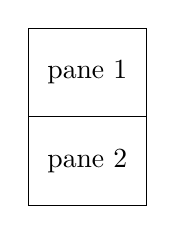
\begin{tikzpicture}[x=1.5cm, y=0.75cm]
      \draw (0, 0) -- (1, 0) -- (1, 3) -- (0, 3) -- (0, 0);
      \draw (0, 1.5) -- (1, 1.5);
      \draw (0.5, 0.75) node{pane 2};
      \draw (0.5, 2.25) node{pane 1};
    \end{tikzpicture}
  \end{problemonly}

  \pspace{\newpage}

  \begin{solution} 
    \highlight{Goal:} Maximize \goal{length of frame}.

    \highlight{Define variables:}
    \begin{itemize}[nosep]
    \item \goal{$F$} = length of frame
    \item $w, h$ as shown below
    \end{itemize}
    \begin{center}
      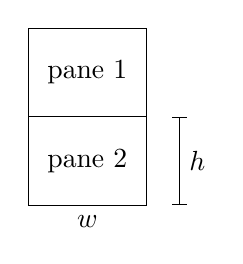
\begin{tikzpicture}[x=1.5cm, y=0.75cm]
        \draw (0, 0) -- node[below]{$w$} (1, 0) -- (1, 3) -- (0, 3) -- (0, 0); %
        \draw (0, 1.5) -- (1, 1.5); %
        \draw (0.5, 0.75) node{pane 2}; %
        \draw (0.5, 2.25) node{pane 1}; %
        \draw[xshift=12pt, |-|] (1, 0) -- node[right]{$h$} (1, 1.5); %
      \end{tikzpicture}
    \end{center}
    \highlight{Formula for goal:} We can see that the three horizontal pieces of frame all have length $w$. The left and right sides of each pane have length $h$, and there are 4 of these in all. So,
    \begin{equation}
      \label{eq:fall2023-fpractice-frame}
      \goal{$F$} = 3w + 4h 
    \end{equation}
    This formula involves both $h$ and $w$, so we need to \highlight{relate $h$ and $w$ using something else we're told in the problem}. 
    \begin{align*}
      \text{area of each pane} &= 300 \\
      wh &= 300 \\
      h &= \frac{300}{w}
    \end{align*}
    Plugging this into (\ref{eq:fall2023-fpractice-frame}) gives the length of the frame in terms of just $w$:
    \[ \goal{$F(w)$} = 3w + \dfrac{1200}{w}\]
    We're also told each pane should be at least 10 inches long and 10 inches wide, which tells us something about the \highlight{domain} of our function. Since we expressed $F$ as a function of $w$, the domain is the possible values of $w$. We're told that $w$ must be at least 10. What's the biggest that $w$ can be? Since each pane needs to have a fixed area, a bigger width corresponds to a smaller height. The smallest possible height is $h = 10$, and when $h = 10$, $w = 30$. So, the largest possible value of $w$ is 30, and the domain of $F(w)$ is $[10, 30]$. 

    \highlight{Critical points:} $\displaystyle F(w) = 3w + 1200 w^{-1}$, so $F'(w) = 3 - 1200 w^{-2} = 3 - \dfrac{1200}{w^2}$. This is undefined when $w = 0$, and it's 0 when
    \begin{align*}
      3 &= \frac{1200}{w^2} \\
      w^2 &= 400 \\
      w &= \pm 20
    \end{align*}
    The only critical point that's in the domain is $w = 20$.

    \highlight{Global maximum:} Since there's only one critical point in the domain, we can try the First or Second Derivative Test. Let's try the Second Derivative Test, since it's easy to calculate that $F''(w) = 2400 w^{-3} = \dfrac{2400}{w^3}$. Then, $F''(20) = \dfrac{2400}{20^3} > 0$, so $w = 20$ is a local minimum. But wait! We wanted a global \emph{maximum}, not a minimum. Since the critical point isn't the global maximum, the global maximum must occur at one of the endpoints of the domain. So, let's plug the endpoints into $F$ to see which gives us the higher value:
    \begin{align*}
      F(10) &= 30 + \frac{1200}{10} = 150 \\
      F(30) &= 90 + \frac{1200}{30} = 130
    \end{align*}
    So, the global maximum is at $w = 10$. Since we found earlier that $h = \dfrac{300}{w}$, the corresponding value of $h$ is $h = \dfrac{300}{10} = 30$. Thus, Karen should make each pane \fbox{10 inches wide and 30 inches tall}. 
  \end{solution} 

\end{enumerate}

\end{document}
